\chapter{Results}
\label{section:results}

This section describes the results of the experiments on the ActivityNet dataset obtained with teh different variations of our architecture.

\section{Evaluation Metric}

In task like classification and detection, the research community and also the ActivityNet Challenge use the same metrics for evaluation to be able to compare results between publications. In our work, we have computed our results using the evaluation scripts provided by the ActivityNet Challenge 2016 organization.

\subsection{Classification Metric}

The classification of videos was assessed with the mean Average Precision (mAP). This is computed as the mean of the Average Precision (AP) of all $M$ classes at the Dataset.

\begin{equation}
	mAP = \frac{1}{M} \sum_{m=1}^{M} AP(m)
\end{equation}

At the same time, the Average Precision for each class is computed based on a ranking of the classes obtained for each video. A Classifier typically predict a confidence score for each of the considered classes, and these scores allow generating these rankings from the most to the less likely class to be depicted by the video. The precision $P$ is the inverse of the position where the correct class appears, and the AP for class $m$ is obtained by averaging all the precision of the videos associated to the class, according to the ground truth. %average of the precision at position $n$, showed as $P(n)$. This precision is defined as the amount of elements in $k_m$ between positions 1 and $n$ in the ranked list divided by $n$.

\begin{equation}
	AP(m) = \frac{1}{K_m} \sum_{n=1}^{k_m} P(n) \cdot rel(n), \text{where } rel(n) = \begin{cases}
        rel(n) = 1 \Leftrightarrow n \in K_m \\
        rel(n) = 0 \Leftrightarrow n \notin K_m \\
\end{cases}
\end{equation}

As an alterative metric, the $Hit@3$ was also considered. In this case the top 3 predictions are considered for each video, considering a good prediction if the correct class is among them. The $Hit@3$ metric simply measure the proportion of videos in the dataset that are correctly predicted under this assumption. This metric has become popular as adopted in the ImageNet image classification challenge.

%\textcolor{red}{XAVI: You should review this definition of AP. I have updated the text but your formula still do not match your text. PLease double check and make sure you understand. ALBERTO: Done}

\subsection{Detection Metric}

For the other task of the Challenge, the temporal localization or detection as the Challenge name it, the metric use to verify the results given is the Mean Average Prediction previously described. But for this task there is a little difference and consist on taking a prediction as correct before computing the mAP when the Intersection over Union (IoU) is higher than a threshold $\alpha$. For the ActivityNet Challenge $\alpha$ value used is $0.5$.
%the Intersection Over Union (IoU). This metric computes a prediction as correct if the IoU of the prediction with the ground truth annotations is higher than a value $\alpha$. Then the mAP is computed. For the ActivityNet Challenge the $\alpha$ value used is 0.5.

%more than one prediction can be made, and for each prediction giving a the probability of success computed.

%\textcolor{red}{XAVI: I do not really understand how mAP and Top-1 and Top-3 are computed in ActivityNet. I have an intuition but you should double check this and review these definitions and expressions. Maybe you find the definitions in the original ActivityNet paper. It has been an error explaining hit3 on detection task as it is not computed. I have change a bit the text of how the mAP is computed to understand it better.}


\section{Training}

The training of the Recurrent Neural Networks was all done using a 256 batch size and 20 \textit{timesteps} to get a good gradient propagation through the \textit{timesteps} and to fit the most possible data into the GPUs when training.

The optimizer function use was the RMSprop\cite{dauphin2015rmsprop} which is known to work very well for training Recurrent Neural Networks. The RMSprop was set with a value of $\rho$ of 0.9 and $\epsilon$ of $10^{-8}$. The value of the learning rate, as it is explained on Section~\ref{section:training}, was set to $10^{-5}$ for all the experimentation done.

At the weighted loss computation, for the background class was found that its frequency of appearance was 0.4. Different values of $\rho$ were finally tested trying to obtain the best results and finally the $\rho$ was set to $0.3$.

Finally the dropout was set to have a probability of $0.5$ as it is the most frequent value used at the literature\cite{srivastava2014dropout}.
%so it was tested to setup $\rho = 0.6$. The results did present a little improvement so it was decided to even do smaller this value, setting it finally $\rho = 0.3$.

% In order to try to fit the most possible data into the GPUs when training each batch and to get a good gradient propagation along the batch's sequence length, for all the experiments done on this project, the batch size was 256 and the timesteps 20.

%\textcolor{red}{XAVI: This section is so small that you may merge it with its counterpart in the Methodology section. It will be much easier to understand if you explain everything in the same section. ALBERTO: I think that on this section I should only give the values set for training as is done in all the publications}

\section{Classification Task}

The first experiments were related to the depth of the network.
%The way to measure the performance, was computing the mAP for the classification task. The different experiments
It was tested from a 3 layers LSTM with 1024 cells each layer, to a one single layer with 512 cells, going through a two layers network with 512 LSTM cells each one.
%All the architectures presented a batch normalization after the input entrance and dropout before and after the LSTM layers. XAVI: You already explained this
Also all the experiments were done exclusively with the features extracted from the C3D network.
Table~\ref{table:classification_by_architecture} shows how the simplest RNN achieved the best performance. This results was because all the networks presented high learning capacity over our data and it was observed a little over-fitting with the deeper architectures.
%\textcolor{red}{XAVI: Did we expect it ? As far as I know, deeper is better... but you may over-fit. Is this maybe the problem ? ALBERTO: I have just said it. }

\begin{table}[H]
\begin{center}
\begin{tabular}{|l|c|c|}
\hline
Architecture & mAP & Hit@3 \\
\hline\hline
3 x 1024-LSTM & 0.5635 & 0.7437 \\
2 x 512-LSTM & 0.5492 & 0.7364 \\
1 x 512-LSTM & \bf0.5938 & \bf0.7576 \\
\hline
\end{tabular}
\end{center}
\caption{Results for classification task comparing different deep architectures. All values with
         only video features on the validation dataset.}
\label{table:classification_by_architecture}
\end{table}

Once the single layer architecture was selected, the network was trained comparing the input features used and also comparing the basic architecture with the one with feedback.  Table~\ref{table:classification_by_features} shows how the basic architecture  with only video features obtain the best results.
The fail of the feedback architecture may be to the discrepancies of the data use at training and testing. At training, as an input of the previous output it has been use the ground truth, while at testing it has been used the predicted output. The difference between the nature of the data can yield to errors and lower performance~\cite{bengio2015scheduled}. %To solve that it would require to 
%due to instabilities caused by training with the ground truth instances from the previous output\cite{}. % ALBERTO: Bibliography?

Regarding the audio, doing some manual exploration over the videos and its audio tracks, it was been observed that in some cases, the audio was completely unrelated, mostly with music that had no relationship with the activity depicted by the video.

\begin{table}[H]
\begin{center}
\begin{tabular}{|l|c|c|}
\hline
Features used & mAP & Hit@3 \\
\hline\hline
Only video & \bf0.5938 & \bf0.7576 \\
Video w/ audio & 0.5755 & 0.7352 \\
Only video \& feedback & 0.5210 & 0.6982 \\
Video w/ audio \& feedback & 0.5652 & 0.7319 \\
\hline
\end{tabular}
\end{center}
\caption{Results for classification task with the model made by one 512-LSTM. Compare between
         features and feedback on the validation dataset.}
\label{table:classification_by_features}
\end{table}

The ActivityNet Dataset is organized in 200 activities, and these activities are also contained in a taxonomy, in particular, at the leaves of a hierarchical structure.
%. The 200 activities which are annotated all the videos of the dataset and the proposed network predict are the leaf nodes of the taxonomy tree.
On this structure there are 5 top level categories that describe higher level of abstraction: \textit{Eating and drinking activities}, \textit{Sports, Exercise and Recreation}, \textit{Household Activities}, \textit{Socializing, Relaxing and Leisure}, \textit{Personal Care}.
The mean average precision was also computed for these 5 top level activities.
%To do so, all the predicted and ground truth activity labels have been changed by its top level activity and then for each of them computed the Average Precision.
As can be seen on Table~\ref{table:top_level_classification_ap} and Figure~\ref{table:top_level_classification_ap} the \textit{Sports, Exercise and Recreation} have an average precision of $94\%$. This can be explained with the fact that all the features extracted from the videos come from a network which weights were trained to work with a dataset of videos, the Sports1M\cite{KarpathyCVPR14}.

\begin{table}[H]
\begin{center}
\begin{tabular}{|r|c|}
\hline
\textbf{Global Activities} & \textbf{AP} \\
\hline\hline
Eating and drinking Activities & 0.56942 \\
Sports, Exercise, and Recreation & 0.93662 \\
Household Activities & 0.74177 \\
Socializing, Relaxing, and Leisure & 0.76494 \\
Personal Care & 0.59931 \\
\hline\hline
\textbf{Global} (mAP) & 0.72241 \\
\textbf{Global} (Hit@3) & 0.92703 \\
\hline
\end{tabular}
\end{center}
\caption{Mean Average Precision computed for the top level activities of the ActivityNet Dataset. The results are computed over the validation dataset.}
\label{table:top_level_classification_ap}
\end{table}

\begin{figure}[H]
\begin{center}
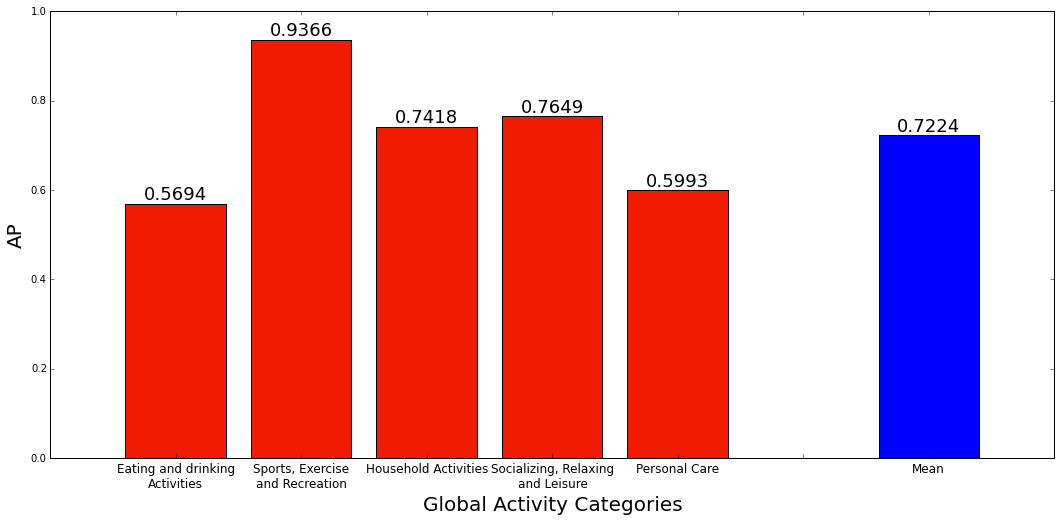
\includegraphics[width=1\linewidth]{img/results/top_activities_classification_ap}
\end{center}
\caption{Representation of the results over the top-level activities}
\label{fig:top_level_classification_ap}
\end{figure}

In addition to the previous figure, and expanding the Average Precision computation to all the activities categories of the Dataset, at Figure~\ref{fig:ap_by_activity_classification} is plot and sorted the Average Precision of all the activities. This plots shows that there is lot of variability in the precision depending on the activity. Taking a closer look, the activities related to sports and require a lot of movement present higher performance in classification. On the other hand, activities more relaxed, which no action happens, tent to have lowest performance.

%\textcolor{red}{XAVI: You did not comment on Figure \ref{fig:map_by_activity_classification}. Add a paragraph about it.}

 %%% Better giving this figure or the one with all the activities and see that mAP varies a lot from one activity to another?
\begin{figure}[H]
\begin{center}
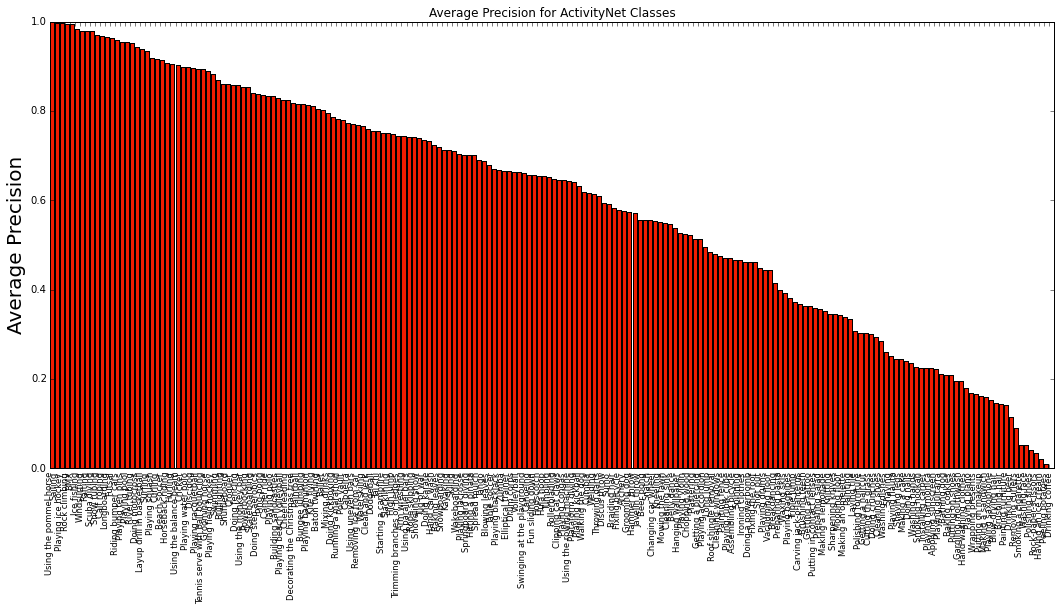
\includegraphics[width=1\linewidth]{img/results/ap_by_activity_classification}
\end{center}
\caption{Average Precision of all the activities of the dataset for the classification task}
\label{fig:ap_by_activity_classification}
\end{figure}

This fact can be perfectly explained with feature extraction used from the videos. It was used a CNN specifically trained for sports videos which always present a lot of action and movement, and this fact may have affected the performance in our network on activities that not present many movement over their video frames.

At the time of submission to the ActivityNet Challenge 2016, the basic architecture was chosen by using the video features only. The results in both validation and test subset are shown in Table~\ref{table:classification_results_challenge}.

\begin{table}[H]
\begin{center}
\begin{tabular}{|l|c|c|}
\hline
Subset & mAP & Hit@3 \\
\hline\hline
Validation & 0.5938 & 0.7576 \\
Test & 0.5874 & 0.7554 \\
\hline
\end{tabular}
\end{center}
\caption{Results of the UPC team at the ActivityNet Challenge 2016 for the classification task.}
\label{table:classification_results_challenge}
\end{table}

As an extra visualization of the results for the classification task, at the Figure~\ref{fig:confussion_matrix} on the Appendix it is attached the confusion matrix of the top-1 activity prediction with the ground truth.



\section{Detection Task}

The main goal of this project is to temporally localize activities on videos. The results obtained are presented in Table \ref{table:detection_architecture_comparison}, considering two architectures: the basic architecture with video features, and the feedback architecture with video and audio features concatenated (this concatenation helped for the classification task, as shown in Table~\ref{table:classification_by_features}).
The basic architecture obtains a slightly better results.

%%%%%%%%
%How I justify the feedback architecture does not give best results than the basic one?
%\textcolor{red}{XAVI: I think you already did earlier, right ? No need to repeat here, or just refer to the same argument exposed before.}
%%%%%%%%

\begin{table}[H]
\begin{center}
\begin{tabular}{|l|c|}
\hline
Architecture & mAP \\
\hline\hline
Basic Architecture & \bf0.22513 \\
Feedback Architecture & 0.20676 \\
\hline
\end{tabular}
\end{center}
\caption{Best results obtain for the temporal activity localization task in the two architectures}
\label{table:detection_architecture_comparison}
\end{table}

The detection task included as post-processing stage described in Section~\ref{section:post_processing}, which aimed at a smoother and better temporal prediction of the activities.
The parameters of this post-processing where also jointly estimated, as shown in Table~\ref{table:detection_postprocessing_comparison}.
These were $\gamma$ as the activity probability threshold, and $k$ as the window size for the mean filter.

\begin{table}[H]
\begin{center}
\begin{tabular}{|l|c|c|c|}
\hline
$\gamma$ & $k=0$ & $k=5$ & $k=10$ \\
\hline
0.2 & 0.20732 & \bf0.22513 & 0.22136 \\
0.3 & 0.19854 & 0.22077 & 0.22100 \\
0.5 & 0.19035 & 0.21937 & 0.21302 \\
\hline
\end{tabular}
\end{center}
\caption{mAP with an IOU threshold of $0.5$ over validation dataset. Here there is a comparison
between values of $k$ and $\gamma$ on post processing.}
\label{table:detection_postprocessing_comparison}
\end{table}

As it can be seen, the best performance was achieved with an activity threshold $\gamma=0.2$ and smoothing filter of $k=5$. The effect of the both of the operations performed after the prediction can be seen in Figures~\ref{fig:smoothing_effect} and~\ref{fig:activty_threshold_effect}. On both figures the temporally location of the activity at the ground truth and at the prediction are displayed, before and after of each of the post-processing.

\begin{figure}[ht]
\begin{center}
%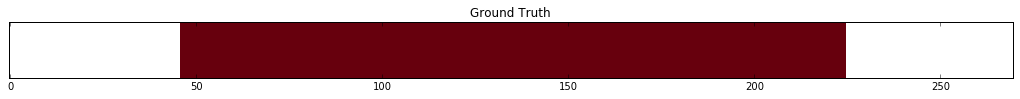
\includegraphics[width=1\linewidth]{img/results/smoothing_effect_1}
%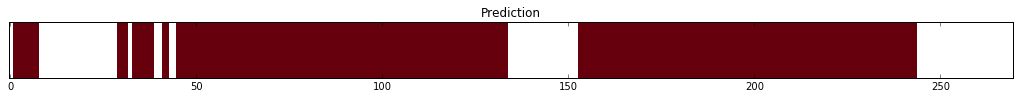
\includegraphics[width=1\linewidth]{img/results/smoothing_effect_2}
%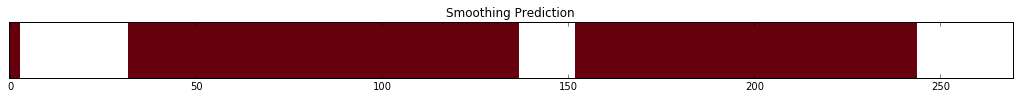
\includegraphics[width=1\linewidth]{img/results/smoothing_effect_3}
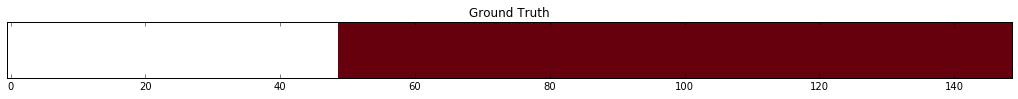
\includegraphics[width=1\linewidth]{img/results/smoothing_effect_4}
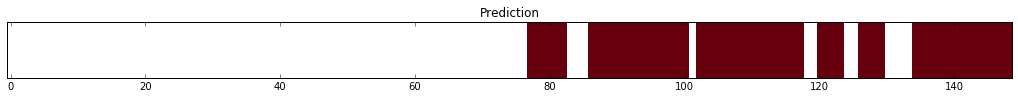
\includegraphics[width=1\linewidth]{img/results/smoothing_effect_5}
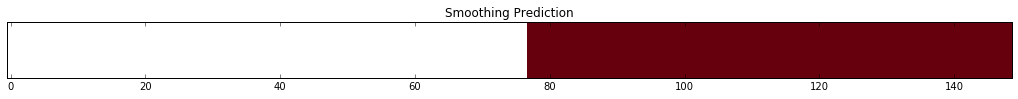
\includegraphics[width=1\linewidth]{img/results/smoothing_effect_6}
\end{center}
\caption{Effect of the mean filter with $k=5$ achieving a smoother activity prediction.}
\label{fig:smoothing_effect}
\end{figure}

\begin{figure}[ht]
\begin{center}
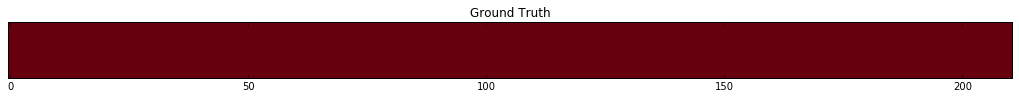
\includegraphics[width=1\linewidth]{img/results/activity_threshold_effect_1}
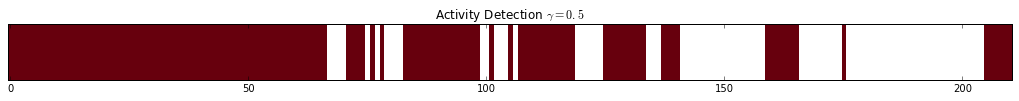
\includegraphics[width=1\linewidth]{img/results/activity_threshold_effect_2}
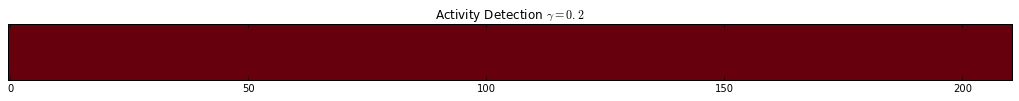
\includegraphics[width=1\linewidth]{img/results/activity_threshold_effect_3}
\end{center}
\caption{Activity Localization using different values of the threshold $\gamma$}
\label{fig:activty_threshold_effect}
\end{figure}

In addition, as it has been done for the classification task, the Average Precision has been computed for the top level activities of the ActivityNet Dataset taxonomy. As can be seen on Table~\ref{table:top_level_detection_ap} and Figure~\ref{fig:top_level_detection_ap}, all the top level activities present a similar precision in activity temporal localization except from the category \textit{Personal Care}, which does not achieve half of the precision of the rest of top level categories. Also notice that the top level category with highest precision is \textit{Sports, Exercise and Recreation}, similarly as in the classification task.

\begin{table}[H]
\begin{center}
\begin{tabular}{|r|c|}
\hline
\textbf{Global Activities} & \textbf{AP} \\
\hline\hline
Eating and drinking Activities & 0.25582 \\
Sports, Exercise, and Recreation & 0.30023 \\
Household Activities & 0.26252 \\
Socializing, Relaxing, and Leisure & 0.26060 \\
Personal Care & 0.11234 \\
\hline\hline
\textbf{Global} (mAP) & 0.23830 \\
\hline
\end{tabular}
\end{center}
\caption{Average Precision of activity localization computed for the top level activities of the ActivityNet Dataset. The results are computed over the validation dataset and with a IoU threshold of 0.5.}
\label{table:top_level_detection_ap}
\end{table}

\begin{figure}[H]
\begin{center}
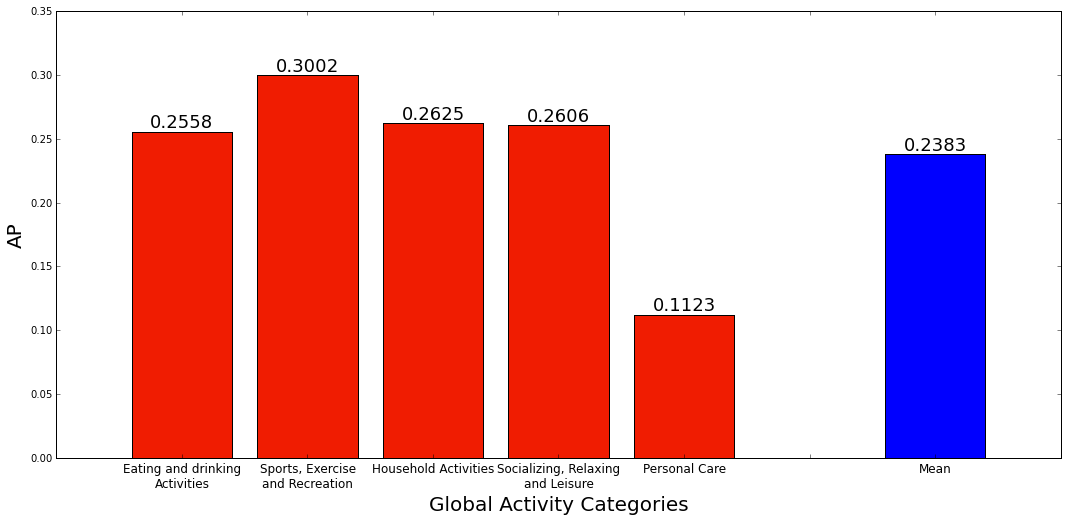
\includegraphics[width=1\linewidth]{img/results/top_activities_detection_ap}
\end{center}
\caption{Representation of the results over the top-level activities}
\label{fig:top_level_detection_ap}
\end{figure}

As it has been done for the classification task, in the Figure~\ref{fig:ap_by_activity_classification} the Average Precision has been plotted for every activity of the dataset. The same effect in the classification task is observe for detection task, where the average precision not performs equally along the activities on the dataset and the more active activities tent to have better results than the more relaxed ones.

\begin{figure}[ht]
\begin{center}
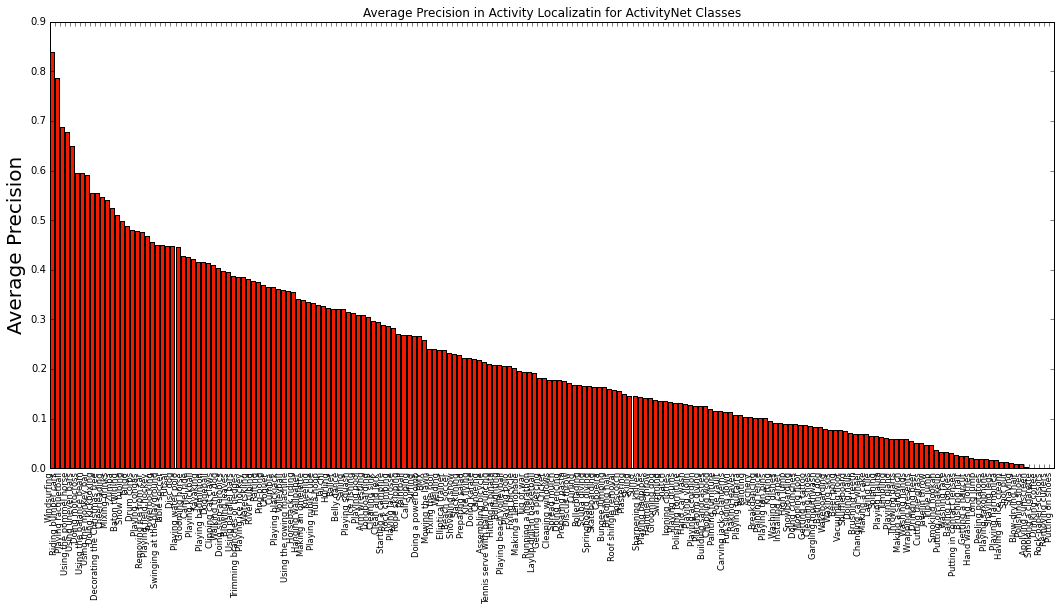
\includegraphics[width=0.8\linewidth]{img/results/ap_by_activity_detection}
\end{center}
\caption{Average Precision of all the activities of the dataset for the detection task}
\label{fig:ap_by_activity_classification}
\end{figure}

It is very common on tasks where the precision is attached to the Intersection over Union computation, to perform the computation for different values of the $\alpha$ threshold of the IoU. On Figure~\ref{fig:map_vs_iou} is plotted the mAP for a rank between 0.1 and 0.5 of the IoU threshold $\alpha$. It can be observed also observed how decreasing the IoU threshold, the mAP increases achieving a value of $0.35$ when the IoU is set to $0.1$.

\begin{figure}[H]
\begin{center}
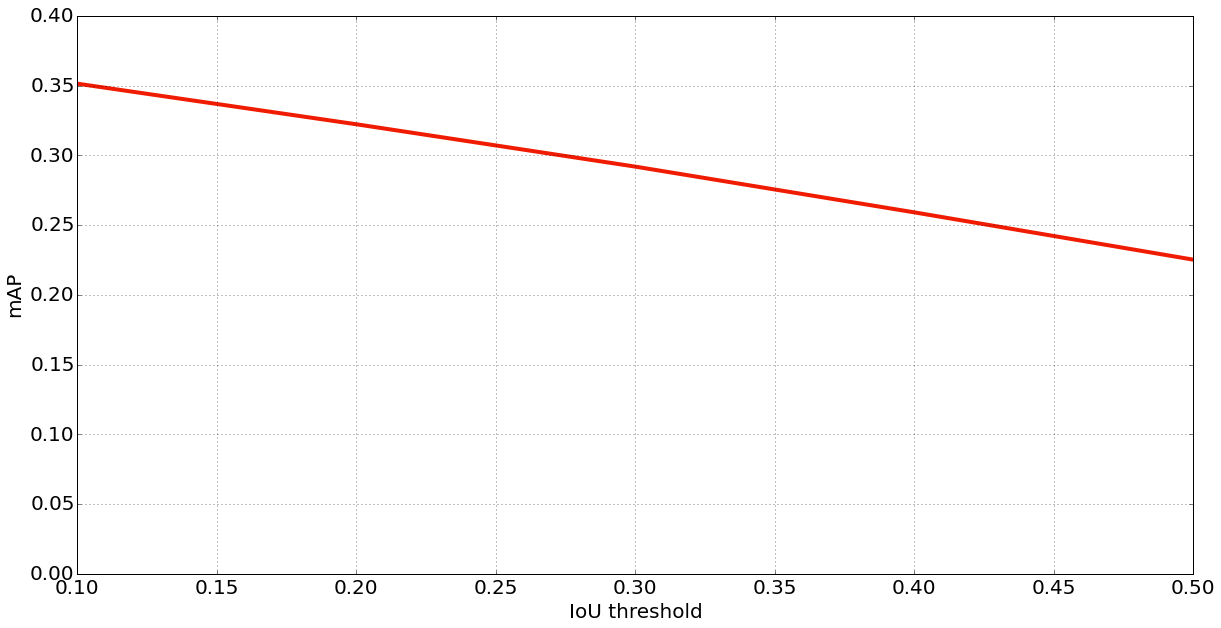
\includegraphics[width=0.8\linewidth]{img/results/map_vs_iou}
\end{center}
\caption{mAP computed against different values of the IoU threshold $\alpha$.}
\label{fig:map_vs_iou}
\end{figure}

Another application the activity localization network proposed in this work is propose temporal regions where activities might be happening. This application is called temporal proposals. Giving only the region where an activity might be happening on the video can be further combined with other networks in parallel to improve the results. It has been set very clear that the aim of this project is to achieve the classification and temporally localization of activities in a very simple and flexible approach.

On the other hand, the performance of the proposed network, used only as a region proposal is plot on Figure~\ref{fig:recall_vs_iou} where the Recall is plot against the IoU threshold.

\begin{figure}[H]
\begin{center}
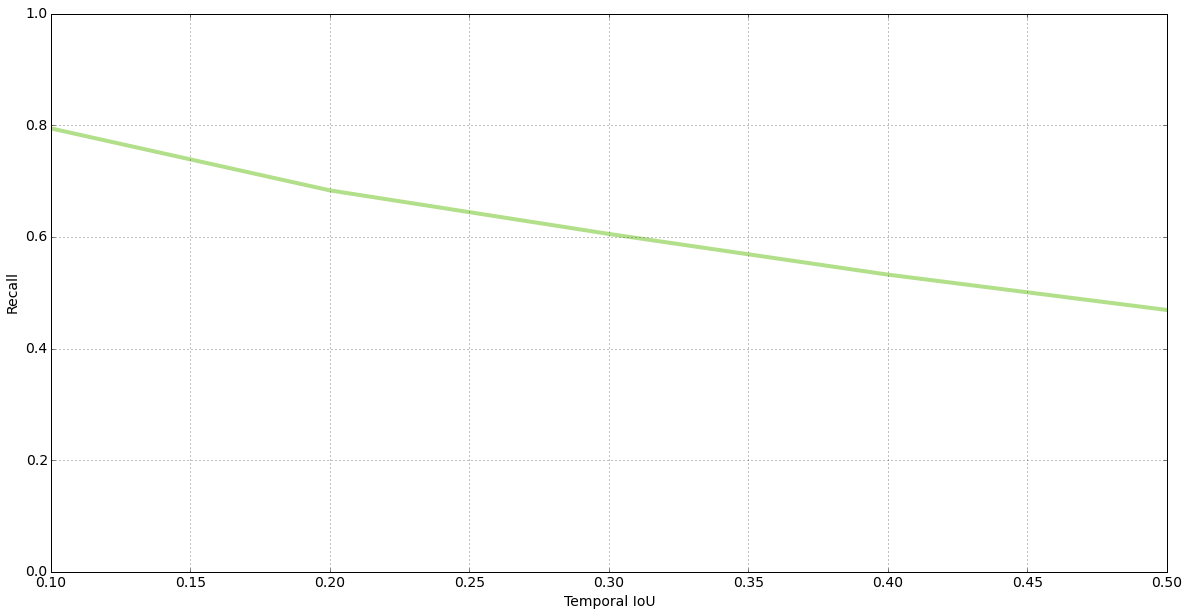
\includegraphics[width=1\linewidth]{img/results/recall_vs_iou}
\end{center}
\caption{Recall of the the temporal regions proposals against different values of the IoU threshold $\alpha$.}
\label{fig:recall_vs_iou}
\end{figure}

%%%%%%%%
%I will put a figure plotting the mAP against the IoU asked between 0.1 and 0.5
%\textcolor{red}{XAVI: Do not forget.}
%%%%%%%%
%Plot with multiple IOU and mAP... And maybe a plot of recall vs IoU threshold to see if the network can create good temporal candidates.


Finally, at the time of submission to the ActivityNet Challenge 2016, the same architecture than in the classification task was chosen. The results in both validation and test subset are shown in Table~\ref{table:detection_results_challenge}.

\begin{table}[H]
\begin{center}
\begin{tabular}{|l|c|c|}
\hline
Subset & mAP \\
\hline\hline
Validation & 0.22513 \\
Test & 0.22369 \\
\hline
\end{tabular}
\end{center}
\caption{Results of the UPC team at the ActivityNet Challenge 2016 for the detection task.}
\label{table:detection_results_challenge}
\end{table}

\section{Qualitative evaluation}

The behavior of the presented model is further analyzed with some qualitative results shown in Figure~\ref{fig:results_visualization_classification}. It presents some examples for classification task, showing the top 3 activities predicted for the each video. Analogously, Figure~\ref{fig:results_visualization_detection} includes a plot the activity detection in time.

Taking a look into the results presented, it can be observed how the classification prediction despite not always being the correct one, it predicts a very similar and related activity which share environment or have very similar action. In addition to this, when the activity require to be temporally localize, sometimes the prediction are not correct due to unsuccessful classification. Furthermore the prediction sometimes presents a lot of variation predicting multiple activity segments for a single ground truth annotation while, on the other hand, the prediction is more conservative when the annotation has multiple temporal segments and the prediction of the proposed network encapsulate them all in a single segment predicted.

Finally, even though the challenge required to temporally localize one single activity per video, the proposed network is capable of predicting multiple classes of activities in a video, just by considering the most probable activity after the smoothing filter.
%With this process, the prediction is a sequence of activities that can be process into multiple temporal activities localization in a single video.
Figure~\ref{fig:results_visualization_detection_classes} shows a case of multiclass activity detection, which proves our claim.
Notice that this multiclass scenario was not considered for the ActivityNet challenge, so no videos nor annotations are available for its evaluation.
%how a multiclass detection would be the prediction. In some cases can be seen how more than one activity class is predicted and would require more exploration over the dataset to check if the predictions may have any sense.

%\textcolor{red}{XAVI: All examples you show are perfect. It would be nice to find some "error" that maybe you could explain why the model is confused. Otherwise the examples are a bit boring :)}

\begin{figure}[H]
\centering
\begin{subfigure}[b]{.4\textwidth}
  \texttt{Video ID: ArzhjEk4j\_Y \\
  Activity: Building sandcastles \\
  \\
  Prediction: \\
  0.7896	Building sandcastles \\
  0.0073	Doing motocross \\
  0.0049	Beach soccer \\}
\end{subfigure}%
\begin{subfigure}[b]{.6\textwidth}
  \centering
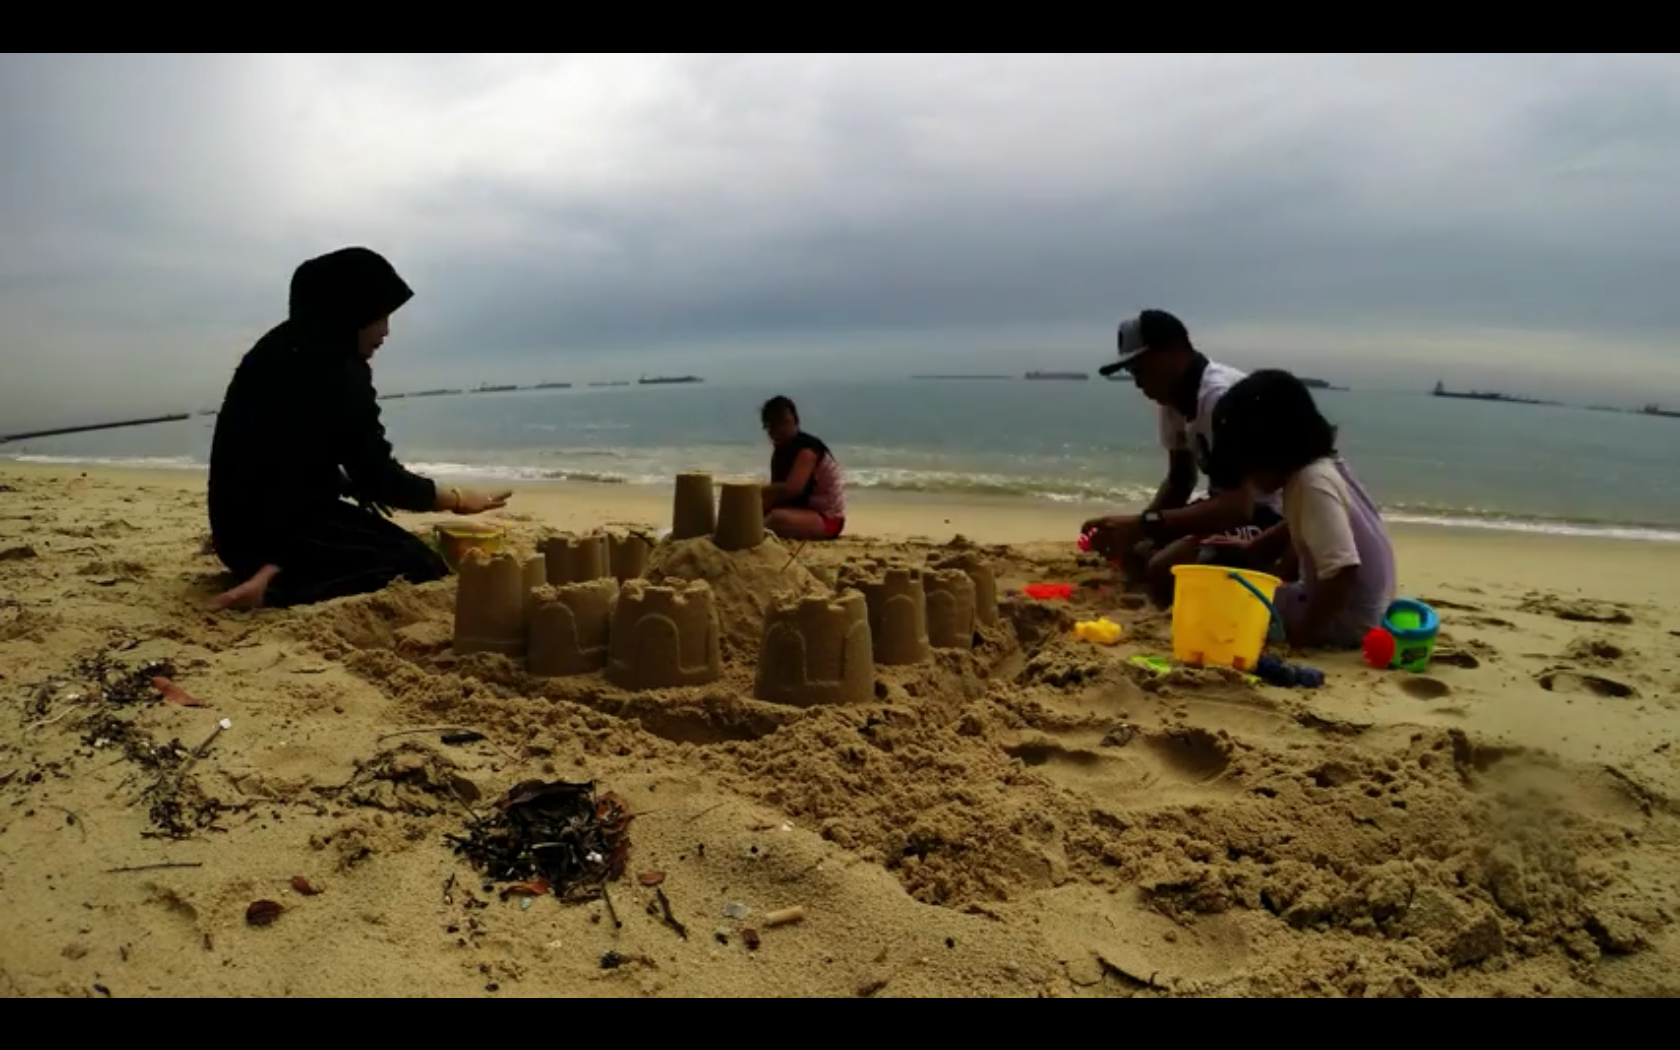
\includegraphics[width=0.95\linewidth]{img/results/results_visualization_classification_1}
\end{subfigure}

\begin{subfigure}[b]{.4\textwidth}
  \texttt{Video ID: AimG8xzchfI \\
	Activity: Curling \\
    \\
    Prediction: \\
    0.3843	Shoveling snow \\
    0.1181	Ice fishing \\
    0.0633	Waterskiing \\}
\end{subfigure}%
\begin{subfigure}[b]{.6\textwidth}
  \centering
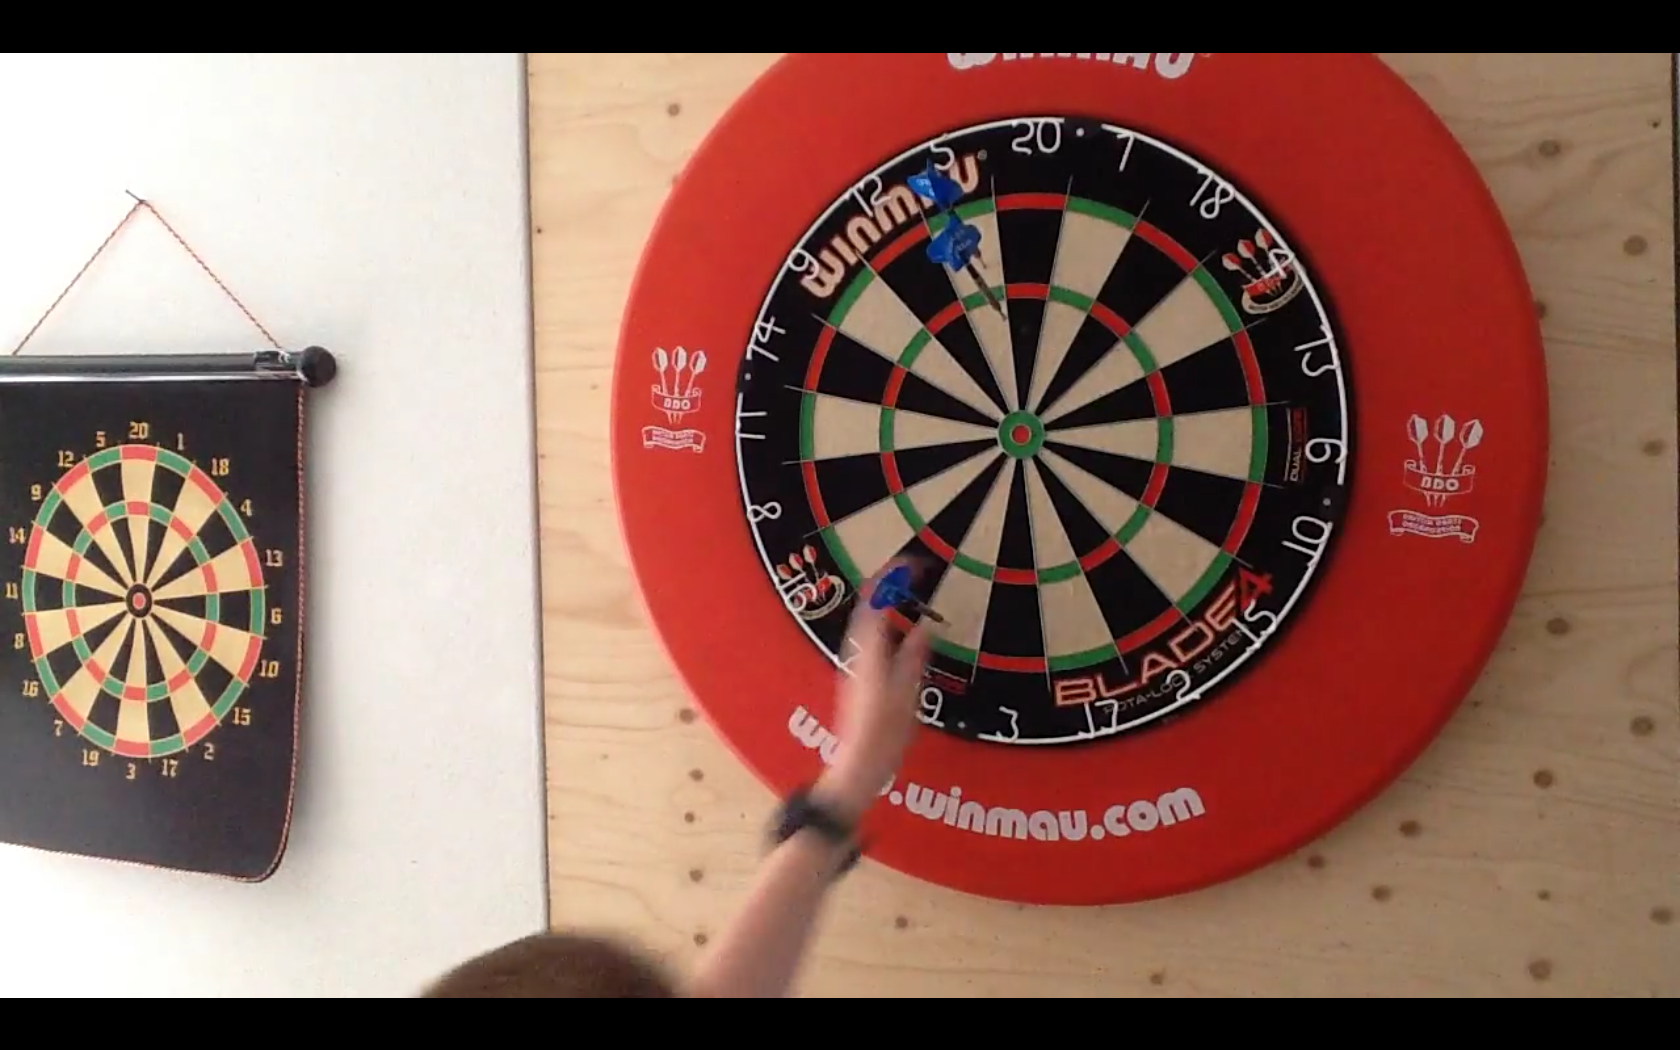
\includegraphics[width=0.95\linewidth]{img/results/results_visualization_classification_2}
\end{subfigure}

\begin{subfigure}[b]{.4\textwidth}
  \texttt{Video ID: q8-iXvYyCGg \\
  Activity: Hopscotch \\
  \\
  Prediction: \\
  0.8477	Running a marathon \\
  0.0231	Triple jump \\
  0.0218	Javelin throw \\}
\end{subfigure}%
\begin{subfigure}[b]{.6\textwidth}
  \centering
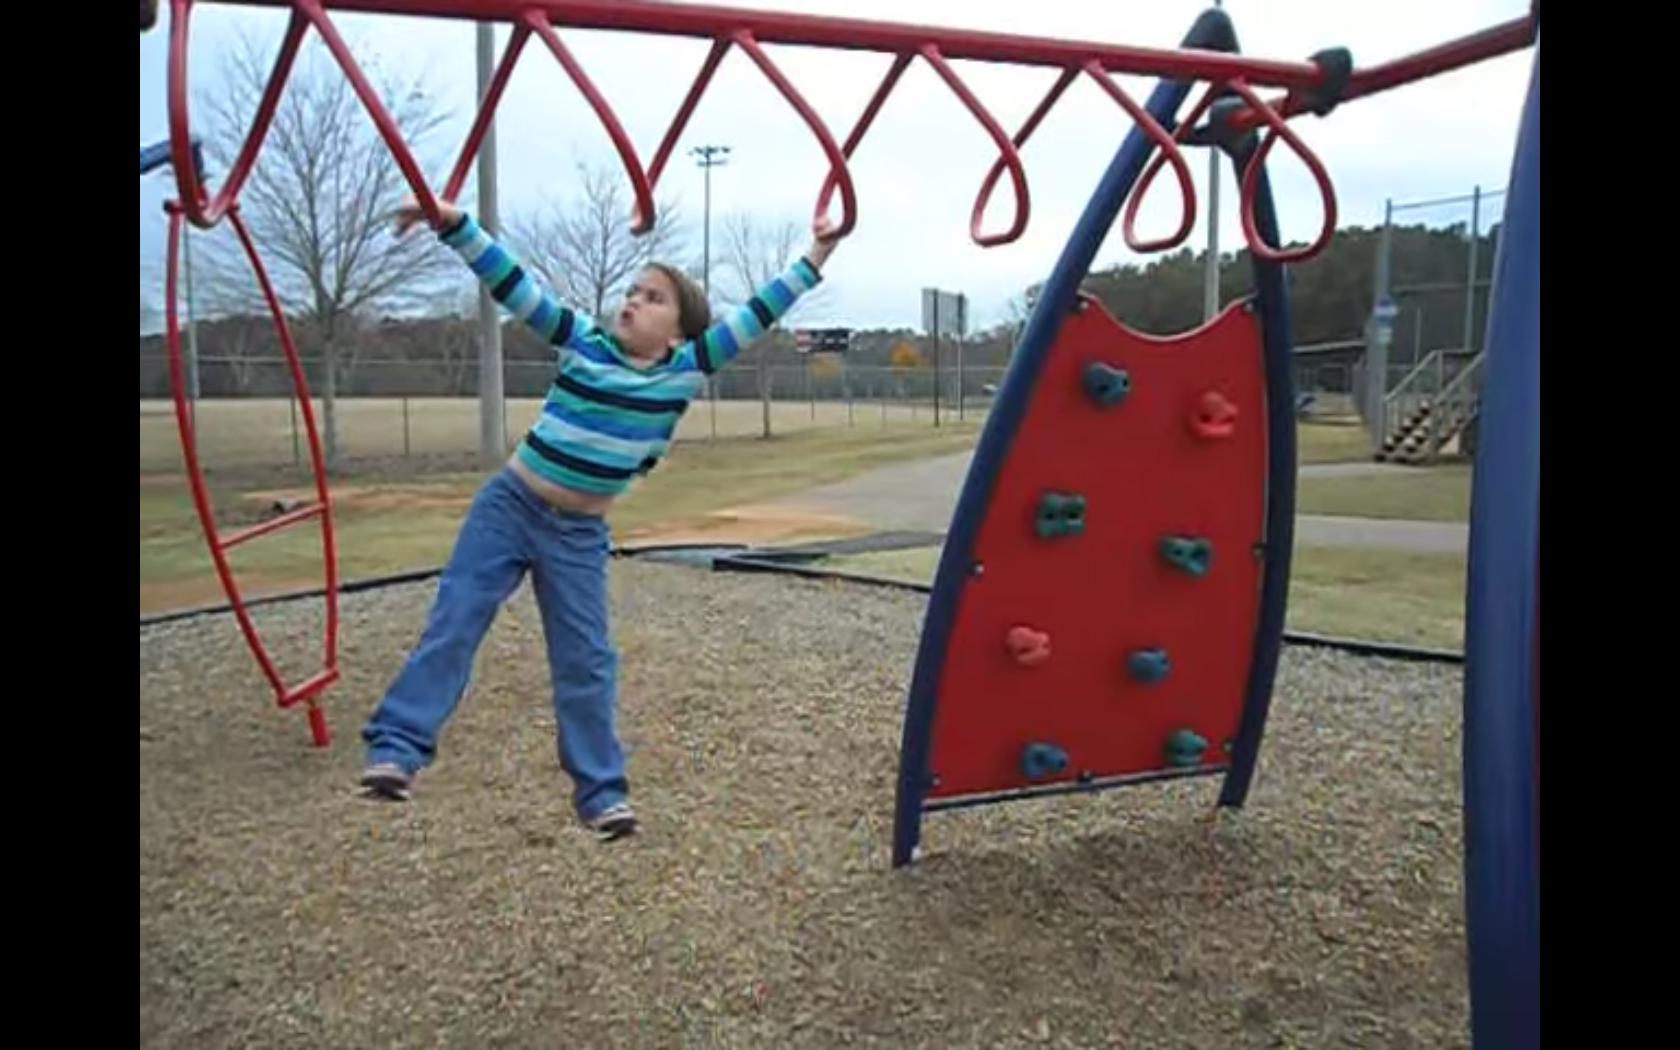
\includegraphics[width=0.95\linewidth]{img/results/results_visualization_classification_3}
\end{subfigure}

\begin{subfigure}[b]{.4\textwidth}
  \texttt{Video ID: VrNHEv6aR38 \\
  Activity: Playing water polo \\
  \\
  Prediction: \\
  0.7645	Playing water polo \\
  0.2018	Swimming \\
  0.0065	Springboard diving\\}
\end{subfigure}%
\begin{subfigure}[b]{.6\textwidth}
  \centering
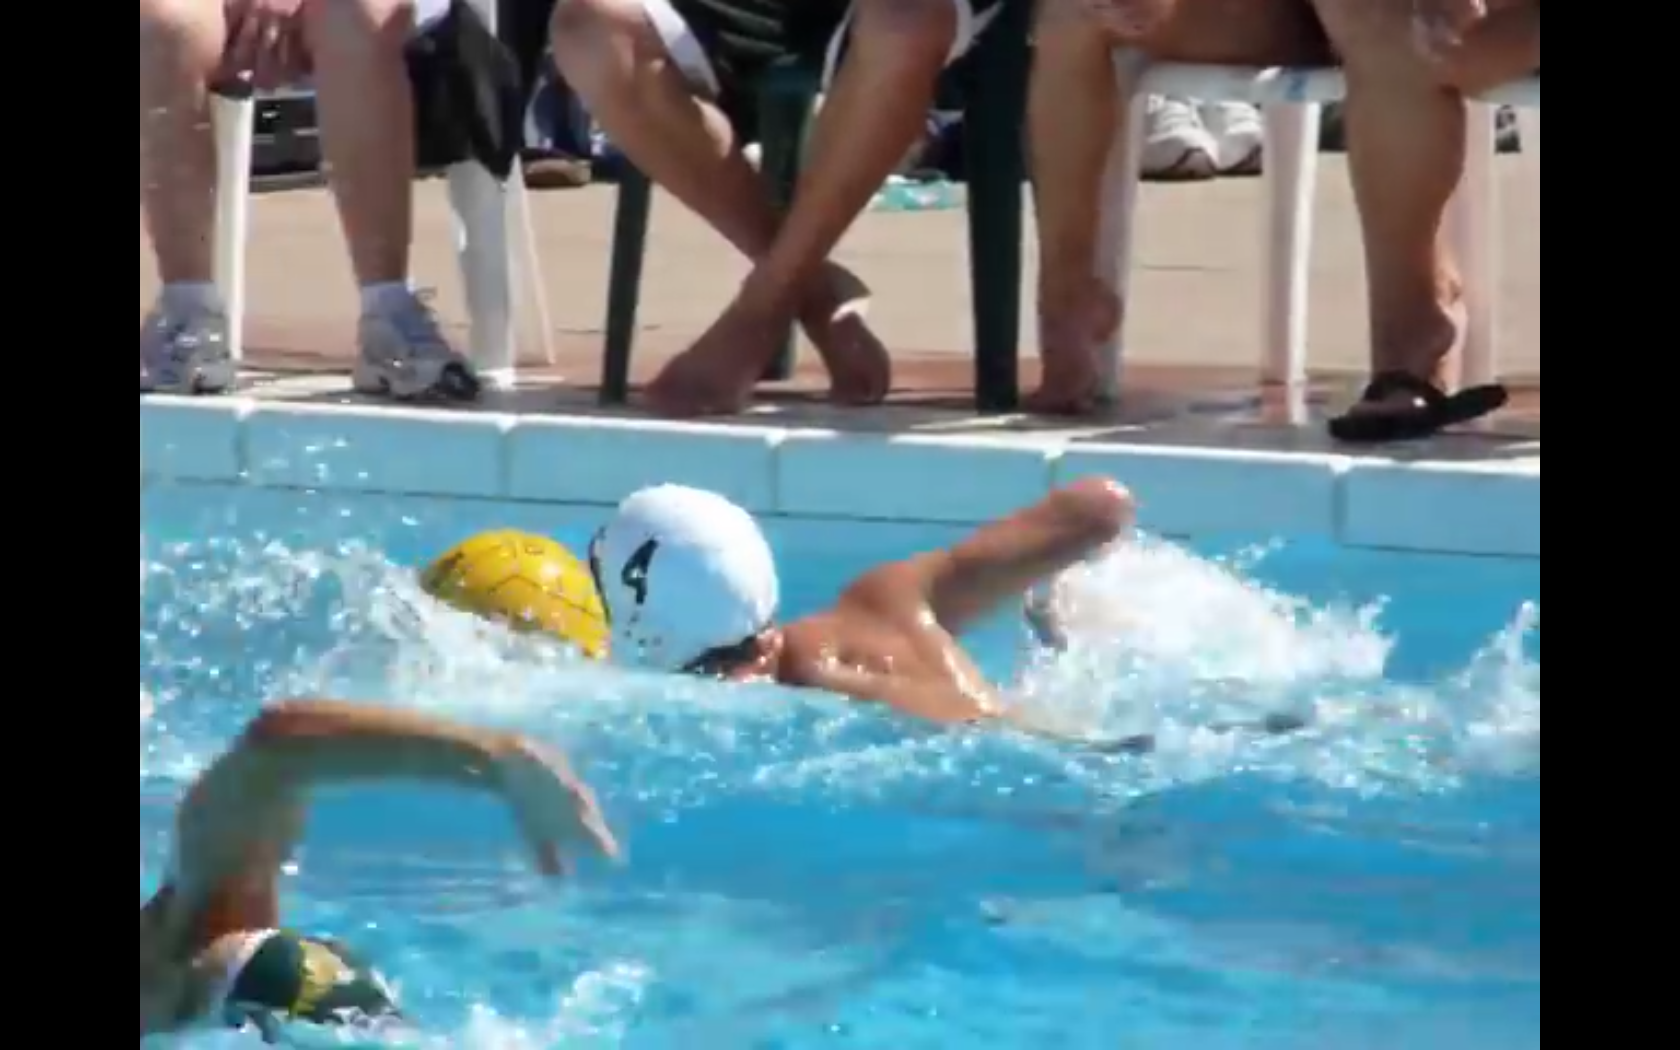
\includegraphics[width=0.95\linewidth]{img/results/results_visualization_classification_4}
\end{subfigure}

\caption{Results for the classification task}
\label{fig:results_visualization_classification}
\end{figure}


%%% I'll put two more examples to fill the page on all this 3 figures.
\begin{figure}[H]
\begin{center}
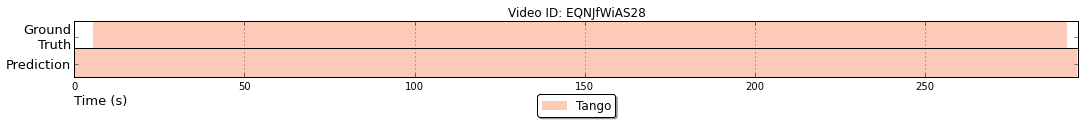
\includegraphics[width=1\linewidth]{img/results/activity_detection/activity_temporal_localization_0}
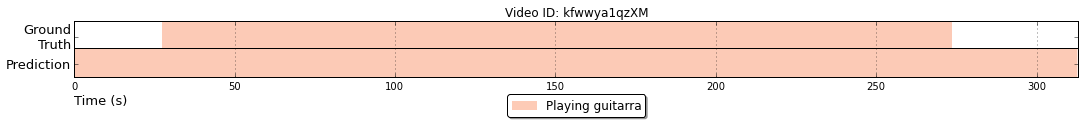
\includegraphics[width=1\linewidth]{img/results/activity_detection/activity_temporal_localization_1}
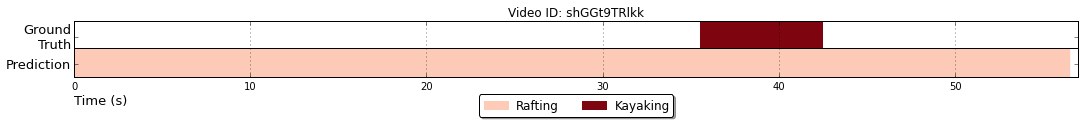
\includegraphics[width=1\linewidth]{img/results/activity_detection/activity_temporal_localization_2}
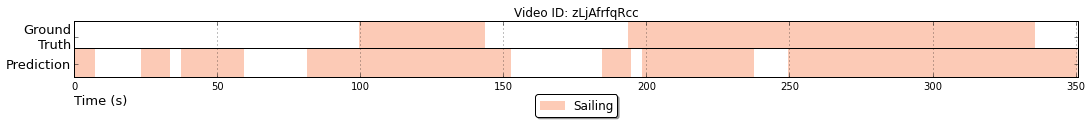
\includegraphics[width=1\linewidth]{img/results/activity_detection/activity_temporal_localization_3}
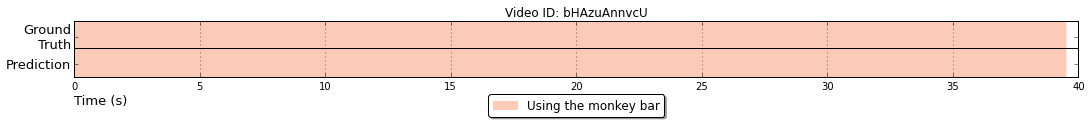
\includegraphics[width=1\linewidth]{img/results/activity_detection/activity_temporal_localization_4}
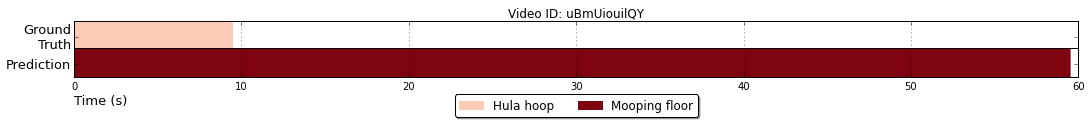
\includegraphics[width=1\linewidth]{img/results/activity_detection/activity_temporal_localization_5}
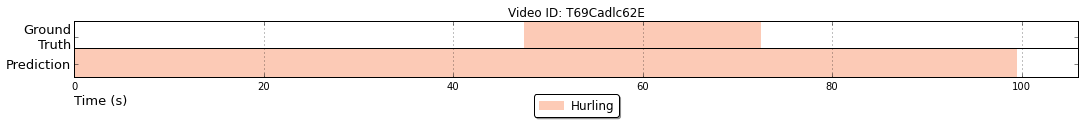
\includegraphics[width=1\linewidth]{img/results/activity_detection/activity_temporal_localization_6}
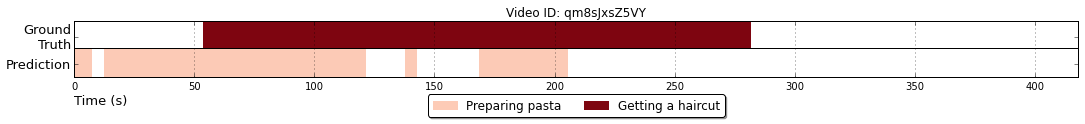
\includegraphics[width=1\linewidth]{img/results/activity_detection/activity_temporal_localization_7}
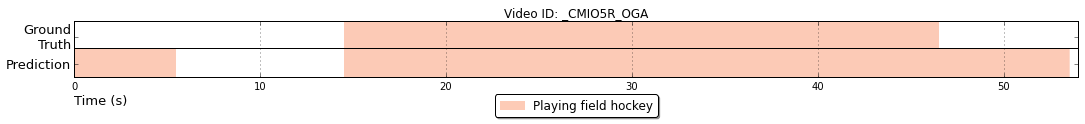
\includegraphics[width=1\linewidth]{img/results/activity_detection/activity_temporal_localization_8}
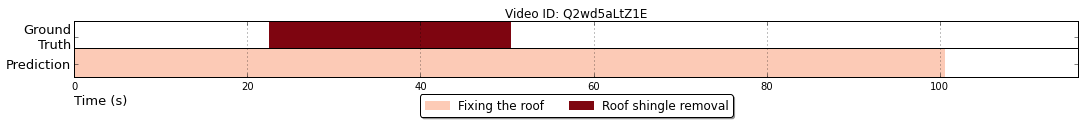
\includegraphics[width=1\linewidth]{img/results/activity_detection/activity_temporal_localization_9}
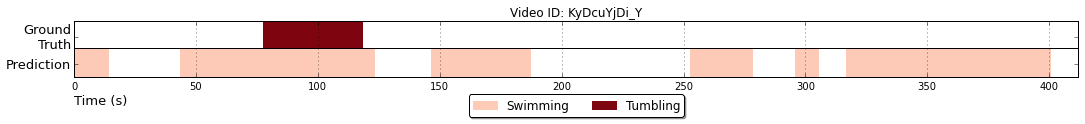
\includegraphics[width=1\linewidth]{img/results/activity_detection/activity_temporal_localization_10}
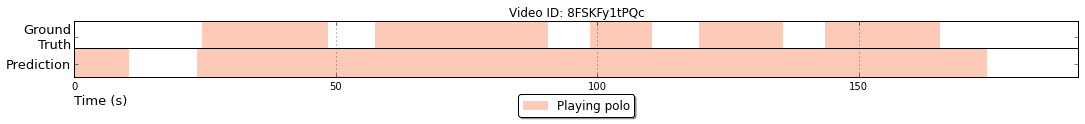
\includegraphics[width=1\linewidth]{img/results/activity_detection/activity_temporal_localization_11}
\end{center}
\caption{Temporal activity localization prediction done by the proposed neural network.}
\label{fig:results_visualization_detection}
\end{figure}

\begin{figure}[H]
\begin{center}
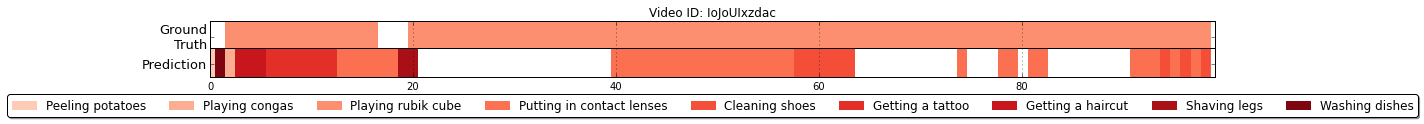
\includegraphics[width=1\linewidth]{img/results/activity_detection_multiple/activity_detection_sample_0}
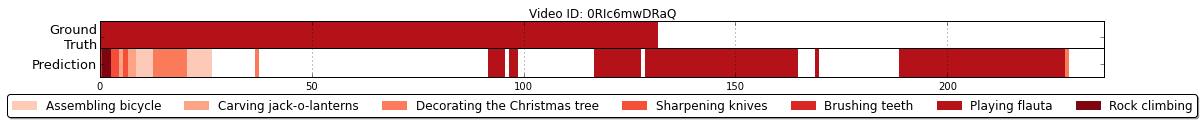
\includegraphics[width=1\linewidth]{img/results/activity_detection_multiple/activity_detection_sample_1}
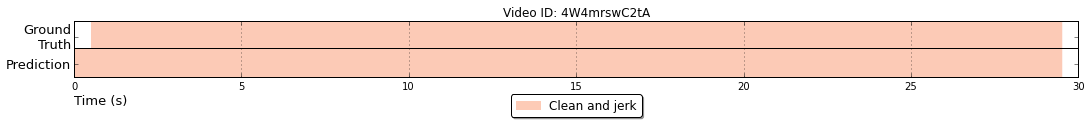
\includegraphics[width=1\linewidth]{img/results/activity_detection_multiple/activity_detection_sample_2}
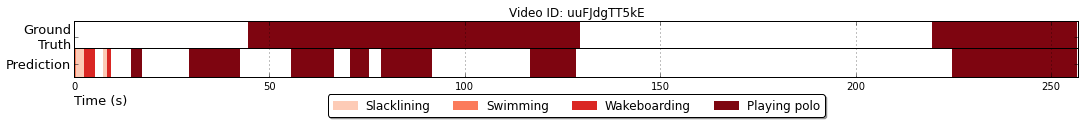
\includegraphics[width=1\linewidth]{img/results/activity_detection_multiple/activity_detection_sample_3}
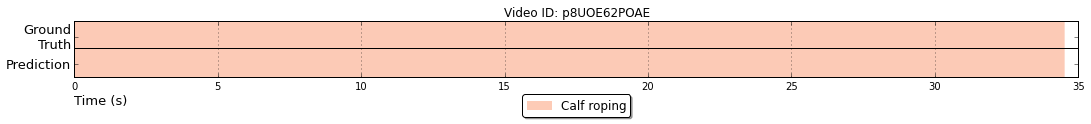
\includegraphics[width=1\linewidth]{img/results/activity_detection_multiple/activity_detection_sample_4}
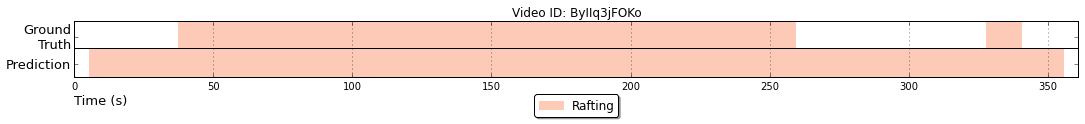
\includegraphics[width=1\linewidth]{img/results/activity_detection_multiple/activity_detection_sample_5}
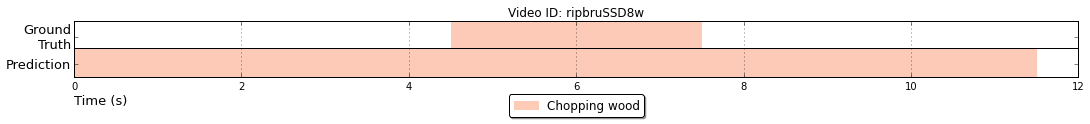
\includegraphics[width=1\linewidth]{img/results/activity_detection_multiple/activity_detection_sample_6}
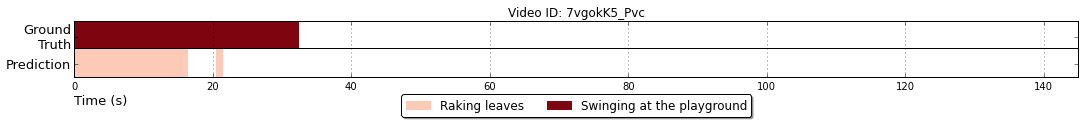
\includegraphics[width=1\linewidth]{img/results/activity_detection_multiple/activity_detection_sample_7}
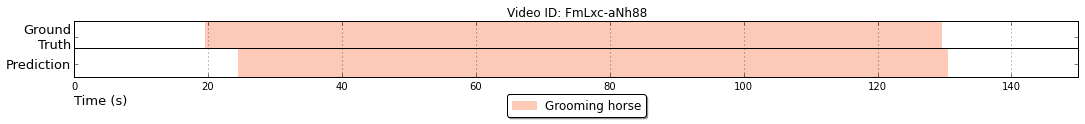
\includegraphics[width=1\linewidth]{img/results/activity_detection_multiple/activity_detection_sample_8}
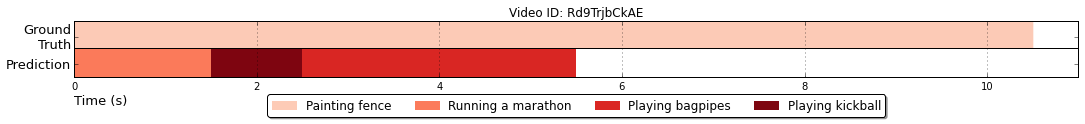
\includegraphics[width=1\linewidth]{img/results/activity_detection_multiple/activity_detection_sample_9}
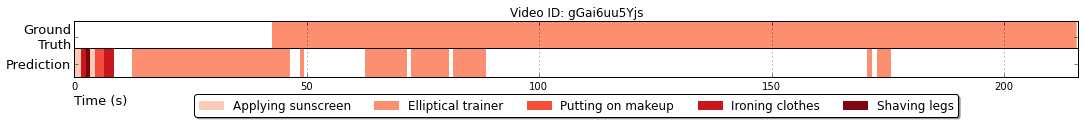
\includegraphics[width=1\linewidth]{img/results/activity_detection_multiple/activity_detection_sample_10}
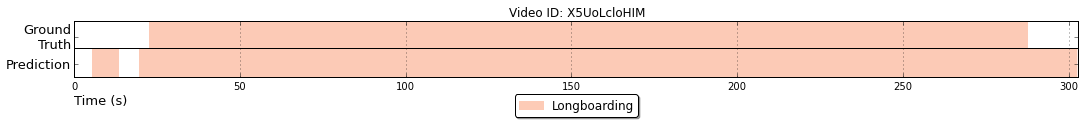
\includegraphics[width=1\linewidth]{img/results/activity_detection_multiple/activity_detection_sample_11}
\end{center}
\caption{Activity predicted from video doing non maximum suppression at each video clip. Different colors represents different activity classes.}
\label{fig:results_visualization_detection_classes}
\end{figure}
